\documentclass[a4paper,11pt,twoside]{article}
%\documentclass[a4paper,11pt,twoside,se]{article}

\usepackage{UmUStudentReport}
\usepackage{verbatim}   % Multi-line comments using \begin{comment}
\usepackage{courier}    % Nicer fonts are used. (not necessary)
\usepackage{pslatex}    % Also nicer fonts. (not necessary)
\usepackage[pdftex]{graphicx}   % allows including pdf figures
\usepackage{listings}
\usepackage{pgf-umlcd}
%\usepackage{lmodern}   % Optional fonts. (not necessary)
%\usepackage{tabularx}
%\usepackage{microtype} % Provides some typographic improvements over default settings
%\usepackage{placeins}  % For aligning images with \FloatBarrier
%\usepackage{booktabs}  % For nice-looking tables
%\usepackage{titlesec}  % More granular control of sections.

% DOCUMENT INFO
% =============
\department{Department of Computing Science}
\coursename{C Programming and Unix 7.5 p}
\coursecode{5DV088}
\title{mfind}
\author{Lorenz Gerber ({\tt{dv15lgr@cs.umu.se}} {\tt{lozger03@student.umu.se}})}
\date{2016-10-17}
%\revisiondate{2016-01-18}
\instructor{Mikael Ränner / Filip Åberg / Jonathan Westin / Mattias Åsander}


% DOCUMENT SETTINGS
% =================
\bibliographystyle{plain}
%\bibliographystyle{ieee}
\pagestyle{fancy}
\raggedbottom
\setcounter{secnumdepth}{2}
\setcounter{tocdepth}{2}
%\graphicspath{{images/}}   %Path for images

\usepackage{float}
\floatstyle{ruled}
\newfloat{listing}{thp}{lop}
\floatname{listing}{Listing}



% DEFINES
% =======
%\newcommand{\mycommand}{<latex code>}

% DOCUMENT
% ========
\begin{document}
\lstset{language=C}
\maketitle
\thispagestyle{empty}
\newpage
\tableofcontents
\thispagestyle{empty}
\newpage

\clearpage
\pagenumbering{arabic}

\section{\textit{mfind} and Thread Safety} 

The scheme in figure \ref{fig:scheme} shows the most important aspects of the mfind
system and how it was implemented here. It can be basically seen as a
producer-consumer system, however, each thread can be both producer
and consumer. The most important source of synchronization is a
semaphore \cite[chapter 15.8] {stevensrago2013} which distributes the jobs to the
threads. When there are no more jobs available, the thread
subsequently terminates. The `do while' loop looks futile on the first
view, however, new jobs can be added after passing the `no wait'
semaphore until checking the value of the semaphore in the `while'
expression which will result in another round to catch a job. 

\begin{figure}
\centering
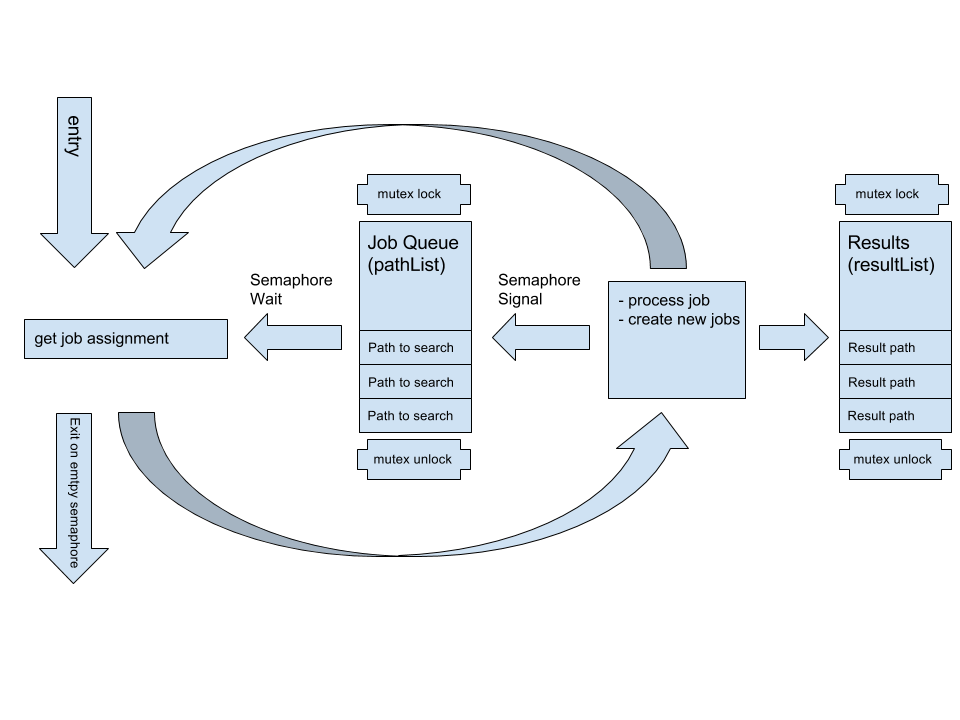
\includegraphics[width=\textwidth]{schema.png}
\caption{\textit{This figure shows a schematic view of the mfind problem.}}
\label{fig:scheme}
\end{figure}

The current construction is thread safe: The last thread in the loop
can not leave until all jobs, also freshly self created are
processed. In certain cases, this could lead to an uneven
workload as threads can leave while it's still possible that new jobs
are generated. This could be addressed by further synchronizing the
threads, forexample with a mutex. That would however also affect
performance for the most general cases. During testing the current
code, it happend rarely that the distribution of tasks was not even
between the different threads.   


\section{Performance Assessment}
To assess the performance of the presented implementation, it was
batched with the `time' function on itchy.cs.umu.se. As instructed, 2
to 10 threads were run each 10 times on \textit{/pkg/ comsol}. The
results were written into a textfile, that was then imported to R
\cite{rlanguage}, parsed and plotted as shown in figure
\ref{fig:perform}. 
 
\begin{figure}
\centering
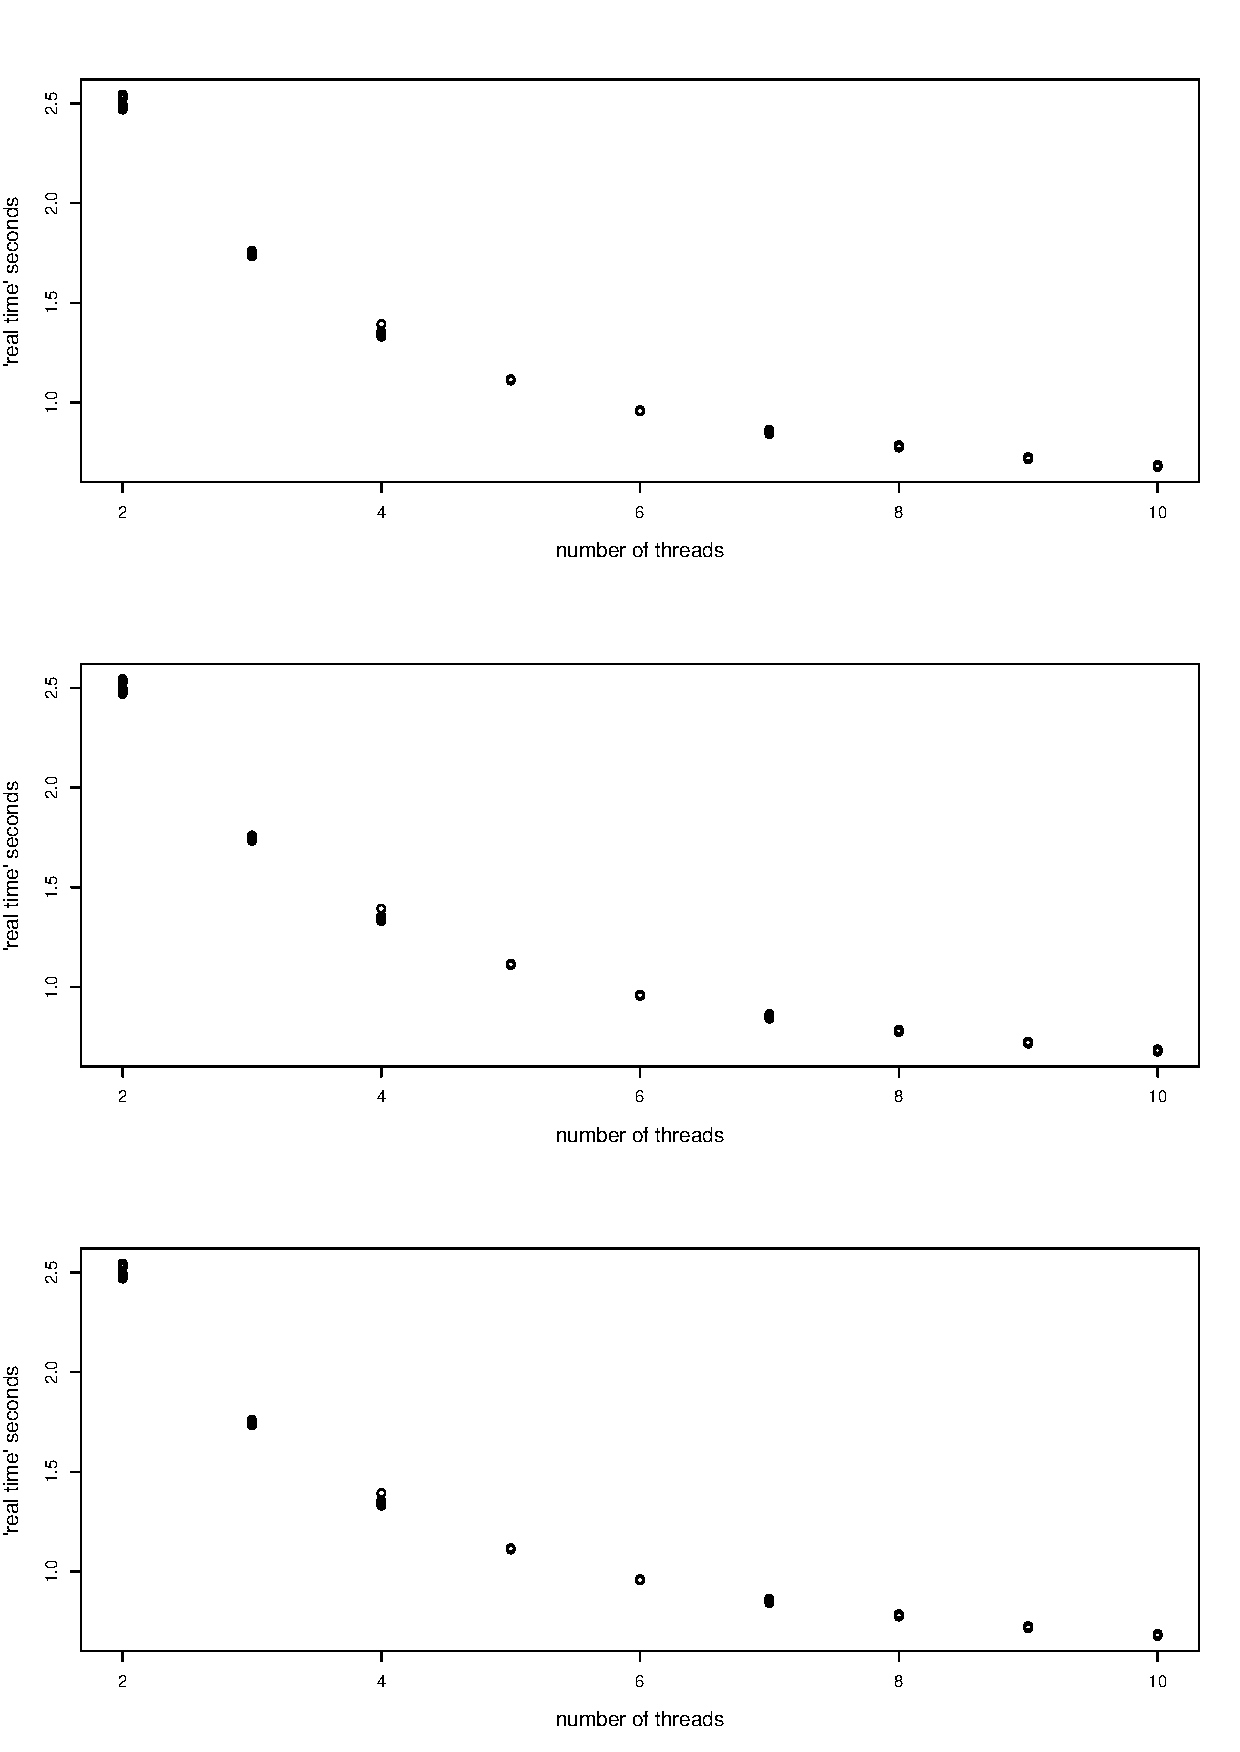
\includegraphics[width=\textwidth]{perform.pdf}
\caption{\textit{This figure shows the execution time in relation to number of threads.}}
\label{fig:perform}
\end{figure}

It was chosen to plot real, user and system time separate. As it can
be seen in uppermost graph of figure \ref{fig:perform}, the `real'
time decreases for increased number of cores. However, it is also
obvious from the plot, that the line flattens out and would eventually
start to increase again when using a too high number of threads. In
single process experiments, it was estimated that the lowest point,
hence the shortest run time is achieved at around 14 threads (not
visible in the graph).

The middle graph shows `user' time which increases steadily, the same
is true for the lowermost graph that shows `system' time. While real
time shows the time which actually passes, `system' and `user' time
account time for each thread used and sum it up. The time increase
correlated with the higher number of threads for `system' and `user'
time shows that more `overhead' time is spend to coordinate the threads.  


\addcontentsline{toc}{section}{\refname}
\bibliography{references}

\end{document}
